\chapter{\difficult{Model theory}}

\section{Simplicial sets}

    \newdef{Simplex category}{\index{simplex!category}
        \nomenclature[S_simpcat]{$\Delta$}{The simplex category.}
        The simplex category $\Delta$ has as objects the posets of the form $[n] = \{0,\ldots,n\}$ and as morphisms the order-preserving maps.
    }
    \newdef{Simplicial set}{\index{simplicial!set}\label{sheaf:simplicial set}
        The category $\mathbf{sSet}$ of simplicial sets is given by the presheaf category $\mathbf{Psh}(\Delta)$. The set $X_n:=X([n])$ is called the set of \textbf{$n$-simplices} in $X$.
    }
    \newdef{Simplicial object}{\index{simplicial!object}
        By internalizing the notion of a simplicial set in any category one obtains the definition of a simplicial object, i.e. a simplicial object in a category $\mathbf{C}$ is a $\mathbf{C}$-valued presheaf on $\Delta$. This way a simplicial set is just a simplicial object in \textbf{Set}.
    }
    \remark{Note that the notion of \textbf{simplicial category} can mean two distinct things. In general it will mean a category enriched in $\mathbf{sSet}$. However, conform the above definition, it can also mean a simplicial object in the (2-)category $\mathbf{Cat}$. It can be shown that all simplicially enriched categories are a specific kind of degenerate simplicial object in $\mathbf{Cat}$.}

    \begin{property}\index{face!map}\index{degeneracy map}
        All morphisms in the simplex category $\Delta$ are generated by two types:
        \begin{itemize}
            \item For every $n$, the unique map $\delta_{n, i}:[n-1]\rightarrow[n]$ which misses the $i^{th}$ element.
            \item For every $n$, the unique map $\sigma_{n, i}:[n+1]\rightarrow[n]$ which duplicates the $i^{th}$ element.
        \end{itemize}
        Under the action of a presheaf this gives the \textbf{face} and \textbf{degeneracy} maps $d_{n, i}$ and $s_{n, i}$. (If the index $n$ is clear, then it is often omitted in the notation.)

        Their fundamental relations are called the \textbf{simplicial identities}:
        \begin{itemize}
            \item $d_i\circ d_j = d_{j-1}\circ d_i$ for $i<j$,
            \item $d_i\circ s_j = s_{j-1}\circ d_i$ for $i<j$,
            \item $d_i\circ s_j = \text{id}$ for $i=j$ or $i=j+1$,
            \item $d_i\circ s_j = s_j\circ d_{i-1}$ for $i>j+1$, and
            \item $s_i\circ s_j = s_{j+1}\circ s_i$ for $i\leq j$.
        \end{itemize}
    \end{property}

    \newdef{Standard simplex}{\index{simplex}\label{sheaf:standard_simplex}
        For every $n$ we define the standard simplicial $n$-simplex $\Delta[n]$ as the Yoneda embedding $\Delta(-, [n])$. We can also define a functor $\func{\Delta_{top}}{\Delta}{Top}$ that maps $[n]$ to the standard topological $n$-simplex $\Delta^n$ (see definition \ref{top:standard_simplex}).
    }
    \begin{property}
        By the Yoneda lemma there exists a natural bijection between the set of $n$-simplices of a simplicial set $X$ and the set of maps $\Delta[n]\rightarrow X$.
    \end{property}

    \begin{construct}[Nerve and realization]
        Consider a general functor $\func{F}{S}{C}$ into a cocomplete category ($\mathbf{S}$ will often be a category of geometric shapes such as the simplex category $\Delta$ or the cube category $\mbox{\mancube}$). Every such functor induces an adjunction
        \begin{gather}
            \mathbf{C}\adj{|-|}{N}\mathbf{Psh}(\mathbf{S}).
        \end{gather}
        The \textbf{realization functor} $|-|$ is defined as the left Kan extension $\text{Lan}_{\mathcal{Y}}F$. The \textbf{nerve functor} is defined as the composition $\mathcal{Y}\circ F^{op}$. (Note that the Yoneda embedding in the definition of the nerve functor is the contravariant version.)

        This definition also holds in an enriched setting, i.e. for  $\mathbf{Psh}(\mathbf{S})\equiv[\mathbf{S}^{op},\mathcal{V}]$. If we furthermore assume that $\mathbf{C}$ is copowered over $\mathcal{V}$, we can express the realization as a coend:
        \begin{gather}
            |X| = \int^{s\in\mathbf{S}}Xs\cdot Fs.
        \end{gather}
    \end{construct}

    \begin{example}[Nerve of a category]\index{nerve}\label{sheaf:nerve}
        \nomenclature[S_Nerve]{$N\mathbf{C}$}{The simplicial nerve of a small category $\mathbf{C}$.}
        To every small category \textbf{C} we can associate a simplicial set $N\mathbf{C}$ in the following way. The set $N\mathbf{C}_0$ is given by the set of objects in $\mathbf{C}$. The set $N\mathbf{C}_1$ is given by the set of morphisms in $\mathbf{C}$. Now, for every two composable morphisms $f, g$ one obtains a canonical commuting triangle. Let $N\mathbf{C}_2$ be the set of all these triangles. The higher simplices are defined analogously. Face maps act by composing morphisms or by dropping the exterior morphisms. Degeneracy maps act by inserting an identity morphism.

        Equivalently, one can define the (simplicial) nerve functor in the following way: Every poset $[n]$ as defined above admits a canonical category structure for which the order-preserving maps give rise to the associated functors. This inclusion $\Delta\hookrightarrow\mathbf{Cat}$ induces the functor
        \begin{gather}
            N:\textbf{Cat}\rightarrow[\Delta^{op},\textbf{Set}]:\mathbf{C}\mapsto\mathbf{Cat}(-, \mathbf{C}).
        \end{gather}
        This way we obtain $N\mathbf{C}_k=\mathbf{Cat}([k], \mathbf{C})$. This object is by definition equivalent to the collection of all strings of $k$ composable morphisms in $\mathbf{C}$.
    \end{example}

    \begin{example}[Geometric realisation]\index{geometric!realisation}
        Consider a simplicial set $X$. From this object one can construct a topological space as follows: First one takes a point for every element in $X_0$. Then one glues 1-simplices between these points using the face maps. The higher simplices are attached analogously.

        For simplicial topological spaces\footnote{These include ordinary simplicial sets since every $n$-simplex $X_n$ can be endowed with the discrete topology.} one can easily give an explicit description:
        \begin{gather}
            |X| := \bigsqcup_{n\in\mathbb{N}}X_n\times\Delta^n / \sim
        \end{gather}
        where the equivalence relation identifies for all morphisms $f\in\text{hom}(\Delta)$ the points $(x, f_*y)$ and $(f^*x, y)$.\footnote{The morphisms $f^*, f_*$ are the ones induced by $X$ and $\Delta_{top}$.} For simplicial sets one can rewrite this as a functor tensor product \ref{cat:functor_tensor_product}:
        \begin{gather}
            |X| = X\otimes_{\Delta}\Delta_{top}
        \end{gather}
        where $\Delta_{top}$ is the embedding $\Delta\hookrightarrow\mathbf{Top}$.
    \end{example}
    \newdef{Singular set}{\index{singular!set}
        Given a topological space $X$ one can also define a simplicial set $\text{Sing}(X)$. Its components are defined as the set of morphisms from the standard (topological) $n$-simplex to $X$:
        \begin{gather}
            \text{Sing}(X)_n := \mathbf{Top}(\Delta^n, X).
        \end{gather}
        This is the object of relevance in the definition of singular (co)homology (see also the Dold-Kan correspondence \ref{sheaf:dold_kan} further below).
    }

    \begin{property}[Classifying space]\index{bar construction}\index{classifying!space}
        For a (discrete) group $G$ one can construct two important objects: the delooping $\mathbf{B}G$ and the classifying space $BG$ (see definitions \ref{cat:group_delooping} and \ref{diff:prin:classifying_space} respectively). As their notations imply there exists some relation between these space: By first taking the nerve of $\mathbf{B}G$ and then going to its geometric realisation we obtain $BG$. In fact this method can be applied to any monoid $A$ to obtain the so-called (two-sided) \textit{bar construction}.
    \end{property}

\subsection{Kan complexes}

    \newdef{Horn}{\index{horn}
        Consider the standard simplex $\Delta[n]$. For all $n\geq1$ and $0\leq k\leq n$ we define the $(n,k)$-horn $\Lambda^k[n]$ as the subsimplicial set obtained by removing the $k^{th}$ face from $\partial\Delta[n]$. When $k=0$ or $k=n$, the horn is said to be \textbf{outer}, otherwise it is said to be \textbf{inner}.
    }

    \newdef{Kan fibration}{\index{Kan!fibration}
        A morphism of simplicial sets that has the right lifting property with respect to all horn inclusions $\Lambda^k[n]\hookrightarrow\Delta[n]$.
    }
    \newdef{Kan complex}{\index{Kan!complex}
        A simplicial set that has all horn fillers or, equivalently, a simplicial set for which the terminal morphism is a Kan fibration.
    }

    \begin{property}[Horn filler condition]
        A simplicial set is the nerve of a (small) category if and only if all of its inner horns admit a unique filler. If we require all horns to admit a unique filler, then we obtain the nerve of a groupoid.
    \end{property}
    By relaxing the above requirements we can generalize the notion of a category (due to \textit{Boardman} and \textit{Vogt}):
    \newdef{Quasicategory\footnotemark}{\index{quasicategory}\index{logos}
        \footnotetext{Some authors such as \textit{Joyal} call these \textbf{logoi} (singular: \textbf{logos}).}
        A simplicial set that has (not necessarily unique) fillers for all inner horns. This condition is sometimes called the \textbf{Boardman condition}.
    }

\subsection{Homological algebra}

    In this section we relate simplicial sets to homological algebra (see chapter \ref{chapter:hom_alg}). A basic introduction is \cite{master2020homology}.

    The objects of focus in this section will be the simplicial vector spaces, i.e. functors $\Delta^{op}\rightarrow\mathbf{Vect}$. Any simplicial set $X:\Delta^{op}\rightarrow\mathbf{Set}$ can be turned into a simplicial vector space through composition with the free vector space functor $F$.

    Given a simplicial vector space $X$, one can construct a chain complex $\mathbf{X}$ as follows:
    \begin{construct}[Alternating face map complex]
        For every $n\in\mathbb{N}$ we define
        \begin{gather}
            \mathbf{X}_n := X_n \equiv X([n]).
        \end{gather}
        The boundary maps $\delta_n$ are defined as an alternating sum of the face maps:
        \begin{gather}
            \delta_n := \sum_{i=1}^n(-1)^id_i.
        \end{gather}
        If we quotient out the degenerate simplices, we obtain the so-called normalized complex.
    \end{construct}
    \begin{theorem}[Dold-Kan correspondence]\index{Dold-Kan correspondence}\label{sheaf:dold_kan}
        The functor mapping simplicial vector spaces to normalized chain complexes gives an equivalence of categories $\mathbf{sVect}\rightarrow\mathbf{Ch}_\bullet(\mathbf{Vect})$.
    \end{theorem}

\section{Localization}

    \newdef{Weak factorization system}{\index{weak!factorization}\label{category:wfc}
        Consider a category $\mathbf{C}$. A pair $(L, R)$ of classes of morphisms in $\mathbf{C}$ is called a weak factorization system (WFS) if it satisfies the folllowing 3 properties:
        \begin{enumerate}
            \item Every morphism in $\mathbf{C}$ factors as a composition $g\circ f$ where $f\in L$ and $g\in R$.
            \item $L$ consists of the morphisms in $\mathbf{C}$ that have the left lifting property \ref{cat:lifting_property} with respect to morphisms in $R$.
            \item $R$ consists of the morphisms in $\mathbf{C}$ that have the right lifting property with respect to morphisms in $L$.
        \end{enumerate}
    }

    \newdef{Homotopical functor}{\index{functor!homotopical}
        Consider two categories with weak equivalences $\mathbf{C, D}$. A functor $\func{F}{C}{D}$ is said to be homotopical if it preserves weak equivalences.
    }

    \newdef{Localization}{\index{localization}\index{homotopy!category}\label{cat:localization}
        Consider a category $\mathbf{C}$ with a collection of morphism $M\subset\text{mor}(\mathbf{C})$. The localization of $\mathbf{C}$ with respect to $M$ is constructed by adding for each morphism $f\in M$ a formal inverse to $\text{mor}(\textbf{C})$. More specifically the localization consists of the following data:
        \begin{enumerate}
            \item a category\footnote{When $\mathbf{C}$ is small, so will its localization. However, even in the case were $C$ is locally small, the localization might be large.} $\mathbf{C}[M^{-1}]$, and
            \item a functor $F_M:\mathbf{C}\rightarrow\mathbf{C}[M^{-1}]$ such that $F_Mf$ is invertible for all $f\in M$
        \end{enumerate}
        such that for every other category $\mathbf{D}$ and functor $\func{F}{C}{D}$, for which $Ff$ is invertible for all $f\in M$, the following conditions are satisfied:
        \begin{itemize}
            \item There exists a functor $Z_F:\mathbf{C}[M^{-1}]\rightarrow\mathbf{D}$ such that $Z_F\circ F_M$ is naturally isomorphic to $F$.
            \item The precomposition functor $F_M^*:[\mathbf{C}[M^{-1}],\mathbf{D}]\rightarrow[\mathbf{C},\mathbf{D}]$ is fully faithfull.
        \end{itemize}
        When $\mathbf{C}$ is a category with weak equivalences $W$, one often calls $\mathbf{C}[W^{-1}]$ the \textbf{homotopy category} $\mathbf{Ho}(\mathbf{C})$. In this context one often denotes the functor $\mathbf{C}\rightarrow\mathbf{Ho(C)}$ by $\gamma_{\mathbf{C}}$.
    }
    \begin{property}
        The localization $\mathbf{C}[M^{-1}]$ is unique up to equivalence.
    \end{property}

    \newdef{Derived functor}{
        Consider a homotopical functor $\func{F}{C}{D}$ and let $\gamma$ be the composition with the localization functor $\gamma_{\mathbf{D}}$. The derived functor $\func{\mathbf{Ho}(F)}{Ho(C)}{Ho(D)}$ is the functor obtained by the universal property of $\mathbf{Ho(C)}$ applied to this composition.

        This definition can be rephrased in terms of Kan extensions: Consider a homotopical functor $\func{F}{C}{D}$ between categories with weak equivalences. The left and right derived functors are defined by Kan extensions:
        \begin{gather}
            LF := \text{Ran}_{\gamma_{\mathbf{C}}}(\gamma_{\mathbf{D}}\circ F)\\
            RF := \text{Lan}_{\gamma_{\mathbf{C}}}(\gamma_{\mathbf{D}}\circ F).
        \end{gather}
        In fact one can drop the assumption that $\mathbf{D}$ has weak equivalences. Then one should simply replace $\gamma_{\mathbf{D}}\circ F$ by $F$ in the above formulas.
    }

\section{Model categories}\label{section:model_categories}

    \newdef{Model structure}{\index{fibration}\index{weak!equivalence}
        Let $C$ be a category. A model structure (in the sense of \textit{Quillen}\footnote{Also called a \textbf{closed model category}.}) on $C$ consists of 3 classes of morphisms
        \begin{enumerate}
            \item \textbf{weak equivalences} $W$,
            \item \textbf{fibrations} $\text{Fib}$, and
            \item \textbf{cofibrations} $\text{Cof}$
        \end{enumerate}
        that satisfy the following two conditions:
        \begin{itemize}
            \item $W$ turns $C$ into a category with weak equivalences (see definition \ref{category:weak_equivalence}).
            \item $(\text{Cof},\text{Fib}\cap W)$ and $(\text{Cof}\cap W,\text{Fib})$ are weak factorization systems on $C$ (see definition \ref{category:wfc}).
        \end{itemize}
    }

    \newdef{Model category}{\index{model!category}\index{category!model|see{model category}}
        A complete and cocomplete category equipped with a model structure.\footnote{\textit{Quillen}'s original definition only required small limits and small colimits.}
    }

    \newdef{Acyclic}{\index{acyclic!fibration}
        The morphisms in $\text{Fib}\cap W$ and $\text{Cof}\cap W$ are said to be \textbf{acyclic} or \textbf{trivial}.
    }

    \newdef{Fibrant object}{\index{fibrant}
        An object in a model category is said to be fibrant if the unique morphism to the terminal object is a fibration. Dually, an object in a model category is said to be cofibrant if the unique morphism from the initial object is a cofibration.
    }
    \begin{property}[Resolution]\index{resolution}
        In a model category the (co)completeness property implies that there exists both an initial and terminal object. The weak factorization property then implies that one can for every object $X$ find a weakly equivalent fibrant replacement $X^f$ and a weakly equivalent cofibrant replacement $X^c$ by suitably factorizing the initial and terminal morphisms. These replacements are also sometimes called \textbf{resolutions} or \textbf{approximations}.
    \end{property}

    \newdef{Proper model}{\index{proper}
        A model category is said to be left proper (resp. right proper) if weak equivalences are preserved by pushouts along cofibrations (resp. pullbacks along fibrations).
    }

    \begin{property}[Model structure on functor categories]\label{cat:model_functor}
        Consider a (small) category $\mathbf{C}$ and model category $\mathbf{D}$. The functor category $[\mathbf{C}, \mathbf{D}]$ admits two model structures:
        \begin{itemize}
            \item \textbf{Injective model structure}: The weak equivalences are the natural transformations that are objectwise weak equivalences and the cofibrations are the natural transformations that are objectwise cofibrations.
            \item \textbf{Projective model structure}: The weak equivalences are the natural transformations that are objectwise weak equivalences and the fibrations are the natural transformations that are objectwise fibrations.
        \end{itemize}
    \end{property}

    \newdef{Quillen adjunction}{\index{Quillen!adjunction}
        Let $\mathbf{C}, \mathbf{D}$ be two model categories. An adjuction \[\mathbf{D}\adj{F}{G}\mathbf{C}\] is called a \textbf{Quillen adjunction} if the left adjoint preserves cofibrations and acyclic cofibrations. It follows from the axioms that this is equivalent to requiring that the right adjoint preserves fibrations and acyclic fibrations. These adjoint functors are called (left and right) \textbf{Quillen functors}.

        If $(F, G)$ is a Quillen adjunction such that for all cofibrant objects $A$ and fibrant objects $B$ the morphism $FA\rightarrow B$ is a weak equivalence if and only if the adjunct morphism $A\rightarrow GB$ is a weak equivalence, then $(F, G)$ is called a \textbf{Quillen equivalence}.
    }

    Quillen equivalences can also be characterized on the level of homotopy categories
    \begin{property}
        Let $L\dashv R$ be a Quillen adjunction. This pair is a Quillen equivalence if and only if The left (resp. right) derived functor of $L$ (resp. $R$) is an equivalence.
    \end{property}

\subsection{Homotopy category}

    \newdef{Homotopy}{\index{homotopy}
        Before we can construct homotopies in general model categories, thereby generalizing the notions from section \ref{section:homotopy}, we have to define the counterpart of the unit interval in a model category $\mathbf{M}$. Consider an object $x\in\ob{M}$. By taking the product and coproduct of two copies of $x$ one can construct the unique diagonal and codiagonal morphisms $\Delta:x\rightarrow x\times x$ and $\nabla:x\sqcup x\rightarrow x$. By factorizing these morphisms using the weak factorization system in $\mathbf{M}$ we obtain two weak equivalences
        \begin{gather}
            x\rightarrow\text{Path}(x)\\
            \text{Cyl}(x)\rightarrow x.
        \end{gather}
        These two objects are called the \textbf{path object} and \textbf{cylinder object} respectively. By choosing them to be a (co)fibration one obtains the notions of \textbf{good} path/cylinder objects.

        Using these objects one can define left and right homotopies between parallel morphisms $f,g:x\rightarrow y$. A left homotopy between $f$ and $g$ is a morphism $\eta:\text{Cyl}(x)\rightarrow y$ such that the following diagram commutes:
        \begin{gather*}
            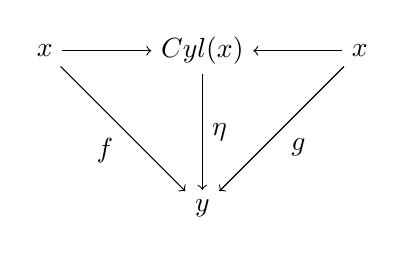
\begin{tikzpicture}
                \node (X) at (-2,0) {$x$};
                \node (X2) at (2,0) {$x$};
                \node (C) at (0,0) {$\text{Cyl}(x)$};
                \node (Y) at (0,-2) {$y$};
                \draw[->] (X) -- (C);
                \draw[->] (X2) -- (C);
                \draw[->] (C) -- node[right]{$\eta$} (Y);
                \draw[->] (X) -- node[below left]{$f$} (Y);
                \draw[->] (X2) -- node[below right]{$g$} (Y);
            \end{tikzpicture}
        \end{gather*}
        A right homotopy between $f$ and $g$ is a morphism $\lambda:x\rightarrow\text{Path}(y)$ such that the following diagram commutes:
        \begin{gather*}
            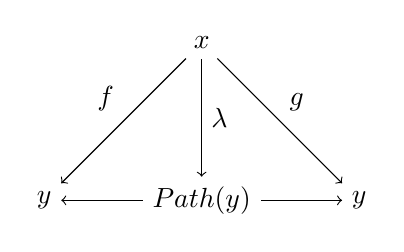
\begin{tikzpicture}
                \node (Y) at (-2,-2) {$y$};
                \node (Y2) at (2,-2) {$y$};
                \node (C) at (0,-2) {$\text{Path}(y)$};
                \node (X) at (0,0) {$x$};
                \draw[<-] (Y) -- (C);
                \draw[<-] (Y2) -- (C);
                \draw[<-] (C) -- node[right]{$\lambda$} (X);
                \draw[<-] (Y) -- node[above left]{$f$} (X);
                \draw[<-] (Y2) -- node[above right]{$g$} (X);
            \end{tikzpicture}
        \end{gather*}
    }

    \begin{property}
        If $x$ is cofibrant, every left homotopy induces a right homotopy. Dually, if $y$ is fibrant, every right homotopy induces a left homotopy.
    \end{property}
    \begin{result}
        Whenever $x$ is cofibrant and $y$ is fibrant, the relations of being left homotopic (or equivalently right homotopic) coincide on $\mathbf{M}(x, y)$ and in particular define equivalence relations. The equivalence classes are denoted by $[x, y]$.
    \end{result}
    \newdef{Homotopy equivalence}{\index{homotopy!equivalence}
        Two objects in a model category are said to be homotopy equivalent if there exists morphisms $f:x\leftrightarrows y:g$ such that $f\circ g$ and $g\circ f$ are homotopic to the identity. The morphisms $f,g$ are then said to be homotopy equivalences.
    }

    In definition \ref{cat:localization} it was shown that one can assign to every category with weak equivalences a ''homotopy category''. When the category has more structure, in this case that of a model category, one can give an equivalent definition:
    \newadef{Homotopy category}{\index{homotopy!category}
        Let $\mathbf{M}$ be a model category. The homotopy category $\mathbf{Ho}(\mathbf{M})$ is the category with the following structure:
        \begin{itemize}
            \item $\ob{Ho(M)}:=\ob{M}$, and
            \item $\text{Hom}_{\mathbf{Ho}(\mathbf{M})}(X, Y) := [X^{cf},Y^{cf}]$.
        \end{itemize}
        In fact we often just restrict to the subcategory of $\ob{Ho(M)}$ on those objects that are fibrant and cofibrant.
    }
    \begin{property}
        The homotopy category of a model category coincides with those of the full subcategories on (co)fibrant objects:
        \begin{gather}
            \mathbf{Ho(M)}\cong\mathbf{Ho(M_f)}\cong\mathbf{Ho(M_c)}\cong\mathbf{Ho(M_{cf})}.
        \end{gather}
    \end{property}

    \begin{theorem}[Whitehead]\index{Whitehead}
        A weak equivalence between objects that are both fibrant and cofibrant is a homotopy equivalence.
    \end{theorem}

    \begin{property}
        If two model categories are Quillen equivalent, their homotopy categories are equivalent.
    \end{property}

    \begin{construct}[Hammock localization]\index{hammock localization}
        Let $\mathbf{M}$ be a model category (in fact this also works for more general categories with weak equivalences) and let $W$ be its collection of weak equivalences. First we can construct its ordinary localization $\mathbf{M}[W^-1]$. Then one can construct the so-called \textit{hammock localization} $L^H\mathbf{M}$. It can be shown that
        \begin{gather}
            \mathbf{Ho}(L^H\mathbf{M}) \cong \mathbf{M}[W^{-1}].
        \end{gather}
        This construction gives a more explicit description of the homotopy category.
    \end{construct}

    \begin{property}[Fundamental category]\index{fundamental!category}
        If $X$ is a quasicategory, then its homotopy category is equivalent to its \textbf{fundamental category}, i.e. the image under the left adjoint of the (simplicial) nerve functor.
    \end{property}

    \newdef{Derived category}{\index{derived!category}
        Consider an Abelian category $\mathbf{A}$ together with its category of chain complexes $\mathbf{Ch}_\bullet(\mathbf{A})$. The derived category $\mathcal{D}(\mathbf{A})$ is defined as the localization of $\mathbf{Ch}_\bullet(\mathbf{A})$ at the collection of quasi-isomorphisms.
    }
    \remark{It can be shown in this case that one can first restrict to the naive homotopy category $\mathbf{K}(\mathbf{A})$, consisting of chain complexes and chain maps up to chain-homotopy, and then localize at the collection of quasi-isomorphisms.}

    In some cases it is useful to consider categories weaker than model categories but stronger than categories with weak equivalences. The best example is given by the full subcategories of a model category on the (co)fibrant objects. These are often easier to handle in the setting of homotopy theory. To formalize this notion we introduce the following definition:
    \newdef{Category of fibrant objects}{\index{fibrant}\index{fibration}
        A category $\mathbf{C}$ with weak equivalences $\mathbf{W}\hookrightarrow\mathbf{C}$ equipped with another subcategory $\mathbf{F}\hookrightarrow\mathbf{C}$, for which the morphisms are called \textbf{fibrations}, such that the following conditions are satisfied:
        \begin{enumerate}
            \item $\mathbf{C}$ admits finite products.
            \item Fibrations and acyclic fibrations are preserved under arbitrary pullbacks.
            \item Every object admits a good path object, i.e. a factorization of the product map $x\rightarrow x\times x$ as the composition of a weak equivalence and a fibration.
            \item All objects are fibrant, i.e. the terminal map $x\rightarrow1$ is a fibration for all objects $x\in\ob{C}$.
        \end{enumerate}
    }

    We now give an important theorem in characterizing when a functor preserves weak equivalences:
    \begin{theorem}[Ken Brown's lemma]\index{Ken Brown}\label{model:ken_brown}
        Let $\mathbf{C}$ be a category of fibrant objects and let $\mathbf{D}$ be a category with weak equivalences. If a functor $\func{F}{C}{D}$ maps acyclic fibrations to weak equivalences, then it preserves all weak equivalences.
    \end{theorem}
    \remark{An analogous theorem exists for categories of cofibrant objects.}

    This lemma allows us to define \dotuline{derived functors} for functors between model categories\footnote{In fact this one is better suited for working in the $\infty$-setting.}:
    \newadef{Derived functor}{\index{derived!functor}
        Let $\func{F}{M}{N}$ be a left (resp. right) Quillen functor. The left (resp. right) derived functors are obtained by postcomposition with the cofibrant (resp. fibrant) replacement functors.
    }

\subsection{Reedy model structure}

    This section is mainly based on \cite{riehl_verity_reedy}.

    Consider a complete and cocomplete category $\mathbf{M}$ (in the remainder of this section we will often take $\mathbf{M}=\mathbf{sSet}$). For any full subcategory $\mathbf{D}\hookrightarrow\mathbf{C}$ we obtain an induced \textbf{truncation} functor\footnote{Sometimes this is called the \textbf{restriction} functor.} $\text{tr}:\mathbf{M}^\mathbf{C}\rightarrow\mathbf{M}^\mathbf{D}$. The left and right adjoints of this functor are respectively called the \textbf{skeleton} and \textbf{coskeleton} functors.
    \begin{formula}
        The adjoint functors are defined by Kan extensions and hence we can express them in terms of (co)ends and weighted (co)limits:
        \begin{gather}
            \text{sk}(X)c := \int^{d\in\ob{D}}\mathbf{C}(d, c)\cdot Xd = \colim^{\text{tr}(\mathbf{C}(-, c))}\\
            \text{cosk}(X)c := \int_{d\in\ob{D}}[\mathbf{C}(c, d), Xd] = \wlim{\text{tr}(\mathbf{C}(c, -))}X.
        \end{gather}
    \end{formula}
    \newdef{Skeletal sets}{\index{skeleton}
        Let $\mathbf{M}=\mathbf{sSet}$ and consider the inclusion $\Delta_{\leq n}\hookrightarrow\Delta$ where the former category is the full subcategory on the objects $\{[0],\ldots,[n]\}$. The $n$-truncation functor $\text{tr}_n$ discards all sets of degree higher than $n$ (or in other words it ''truncates'' a simplicial set at degree $n$).

        The $n$-skeleton functor $\text{sk}_n$ takes a simplicial set $S$ of degree $\leq n$ and freely adds degenerate simplices in degrees $>n$, i.e. it is the smallest simplicial set containing $S$ as a simplicial subset. The $n$-coskeleton functor $\text{cosk}_n$ adds a simplex in degree $>n$ whenever all of its faces are present, i.e. the $m$-simplices in $\text{cosk}_nX$ are given by the collection of all $(m+1)$-tuples of $(m-1)$-simplices that are compatible (along lower simplices).
    }
    \begin{property}[Nerves]
        The nerve functor $\func{N}{Cat}{sSet}$ from definition \ref{sheaf:nerve} is a fully faithful functor to the category of 2-coskeletal simplicial sets.
    \end{property}

    For Reedy categories \ref{cat:reedy} one can also define $n$-truncation, $n$-skeleton and $n$-coskeleton functors by restricting to the full subcategories on elements of degree $\leq n$. In this case we define the following notions:
    \newdef{Matching and latching objects}{\index{matching!object}\index{latching object}
        Let $\mathbf{R}$ be a Reedy category and consider a diagram $X\in\funccat{R}{C}$ where $\mathbf{C}$ is small. Consider the skeleton monad and coskeleton comonads (also often just called the skeleton and coskeleton functors) $\mathbf{sk}_n:=\text{sk}_n\circ\text{tr}_n$ and $\mathbf{cosk}_n:=\text{cosk}_n\circ\text{tr}_n$. The latching and matching objects of $X$ are defined as the restrictions of $\mathbf{sk}_{n-1}$ and $\mathbf{cosk}_{n-1}$ to the degree $n$ subcategory of $R$.

        The counit of the skeleton adjunction and the unit of the coskeleton adjunction give rise to the \textbf{latching} and \textbf{matching} maps.
    }
    \begin{property}
        One can also define the latching and matching objects through (co)limits. Consider the subcategory $R^+(r)$, i.e. the subcategory of $R^+/r$ on all objects except the identity $\mathbbm{1}_r$. The latching object $L_rX$ can then be shown to be isomorphic to the colimit of $X$ over $R^+(r)$.
    \end{property}

    \begin{example}[Simplicial objects]\index{Eilenberg-Zilber}
        The above property enables us to give a nice interpretation to latching objects in the case of $\mathbf{R}=\Delta^{op}$. Using the \textit{Eilenberg-Zilber} lemma one can show that the $n^{th}$ latching object of a simplicial object is given by its collection of degenerate $n$-simplices.
    \end{example}

    \newdef{Boundary}{\index{boundary}
        The boundary of a representable presheaf $\mathbf{R}(-, r)$ is defined as the latching object of the Yoneda embedding $\func{\mathcal{Y}}{R}{Psh(R)}$ at $r$. It is denoted by $\partial\mathbf{R}(-, r)$. It can be shown that $\partial\mathbf{R}(-, r)$ consists of exactly those morphisms that are not in $\mathbf{R}^-$.

        The latching map coincides with the canonical inclusion $\partial\mathbf{R}(-, r)\hookrightarrow\mathbf{R}(-, r)$.
    }
    \begin{formula}
        One can show that the latching and matching objects can be obtained through (co)limits weighted by boundaries:
        \begin{gather}
            M_rX \cong \wlim{\partial\mathbf{R}(r, -)}X\\
            L_rX \cong \colim^{\partial\mathbf{R}(-, r)}X\label{model:latching_boundary}
        \end{gather}
    \end{formula}

    From here on we will also assume $\mathbf{M}$ to be a model category (as was already the case in the previous section). We will define a model structure on the functor category $\funccat{R}{M}$ for Reedy $R$.
    \newdef{Relative matching and latching objects}{
        Consider the (weighted) colimit bifunctor $\func{\text{colim}}{Psh(R)\times[R, M]}{M}$. The \textit{Leibniz construction} (see definition \ref{model:pushout_product} below) allows us to define the relative latching object of $f:X\rightarrow Y$ at $r\in\ob{R}$ as the ''Leibniz colimit'' of the boundary inclusion $\partial\mathbf{R}(-, r)\hookrightarrow\mathbf{R}(-, r)$ and $f$.

        By equations \ref{cat:weighted_hom_colimit} and \ref{model:latching_boundary} the relative latching map is of the form $Xr\sqcup_{L_rX}L_rY\rightarrow Yr$. By suitably dualizing this construction one also gets the relative matching map $Xr\rightarrow Yr\times_{M_rY}M_rX$.
    }

    \begin{property}[Reedy model structure]
        Let $\mathbf{R}$ be a Reedy category and let $\mathbf{M}$ be a model category. The functor category $\funccat{R}{M}$ admits the following model structure:
        \begin{itemize}
            \item The weak equivalences are the levelwise weak equivalences.
            \item The (Reedy) fibrations are those morphisms for which the relative matching map is a fibration (in $\mathbf{M}$) for all $r\in\ob{R}$.
            \item The (Reedy) cofibrations are those morphisms for which the relative latching map is a cofibration (in $\mathbf{M}$) for all $r\in\ob{R}$.
        \end{itemize}
    \end{property}

\subsection{Simplicial spaces}

    A good reference for this section and in particular for the theory of Segal spaces is \cite{rezk}.

    \begin{example}[Topological spaces]
        As a first example we look at the category $\mathbf{Top}$ of topological spaces\footnote{See chapter \ref{chapter:topology} and onwards.}. This category can be endowed with the structure of a model category by taking the weak equivalences to be the weak homotopy equivalences and by taking the fibrations to be the Serre fibrations.
    \end{example}
    \begin{example}[Simplicial sets]
        As a second example we can consider the category $\mathbf{sSet}$ of simplicial sets \ref{sheaf:simplicial set}. This category can be turned into a model category by taking the weak equivalences to be the morphisms that induce weak homotopy equivalence between geometric realisations and by taking the fibrations to be Kan fibrations (fibrant objects are exactly the Kan complexes). The cofibrations are easily seen to be the levelwise injections.
    \end{example}
    \newnot{Quillen model structure}{
        The model structure defined in the above example is generally called the \textit{Quillen}-model structure on simplicial sets (since he was the first one to define it) and it is denoted by $\mathbf{sSet}_{Quillen}$.
    }
    \begin{property}\label{cat:quillen_sset_top}
        The adjoint pair of geometric realisation and singular set functors gives a Quillen equivalence between the above model categories. This result enables us to look at simplicial sets as if they were spaces and vice versa. Most of homotopy theory can be done in either categories.
    \end{property}
    \begin{property}
        Equivalent categories have weakly equivalent nerves.
    \end{property}
    The converse is not true:
    \remark{Because the information in nerves is not sufficient to distinguish between categories (and groupoids) since information about things such as invertibility is lost, i.e. weakly equivalent nerves do not necessarily come from equivalent categories, it is often useful to replace the model structure on $\mathbf{sSet}$ by an alternative one. Instead of taking the Kan complexes to be the fibrant object, \textit{Joyal} and \textit{Lurie} have shown that one can also take the (strictly weaker) quasicategories as fibrant objects to obtain a more informative structure, i.e. weak equivalences can distinguish between (nerves of) categories and groupoids. The fibrations will now be the inner Kan fibrations.}

    \newdef{Dwyer-Kan equivalence}{\index{equivalence!Dwyer-Kan}
        Consider a simplicial functor $\func{F}{C}{D}$ between two simplicial categories. This functor is called a Dwyer-Kan equivalence if
        \begin{itemize}
            \item the induced map on Hom-objects is a weak equivalence. $F$ is also said to be $\infty$-fully faithful,\footnote{This is related to the fact that simplicial categories are models for $\infty$-categories.} and
            \item the induced map on connected components $\pi_0 F:\pi_0\mathbf{C}\rightarrow\pi_0\mathbf{D}$ is an equivalence (of categories).
        \end{itemize}
    }
    \begin{property}
        Quillen equivalent model categories have Dwyer-Kan equivalent simplicial localizations.
    \end{property}

    \begin{example}[Bisimplicial sets]
        One can also look at the simplicial objects in $\mathbf{sSet}$. These are often called bisimplicial sets or \textbf{simplicial spaces}\footnote{The latter name follows from the fact that topological spaces and simplicial sets are (Quillen) equivalent.}. Since $\mathbf{sSet}$ is a model category we know from property \ref{cat:model_functor} above that $\mathbf{ssSet}$ admits itself a model structure. It can furthermore be shown that the injective model structure on $\mathbf{ssSet}$ coincides with the Reedy model structure.\footnote{This is, however, a highly nontrivial statement.}

        This allows us to define the notion of \textbf{Segal spaces}:
    \end{example}
    \newdef{Segal space}{\index{Segal!space}
        Consider a fibrant object $X$ in the injective (or Reedy) model structure on $\mathbf{ssSet}$. This bisimplicial set is called a Segal space if it satisfies the following weak form of the \textit{Segal condition}:
        \begin{gather}
            X_n\xrightarrow{\ \simeq\ }X_1\times_{X_0}\cdots\times_{X_0}X_1
        \end{gather}
        is a weak equivalence for all $n\geq1$. These maps are called \textbf{Segal maps} in general.
    }
    \newdef{Segal category}{\index{Segal!category}
        A bisimplicial set $X$ is called a Segal precategory if $X_0$ is discrete. It is called a Segal category if in addition all its Segal maps are weak equivalences.
    }

    \newdef{Mapping space}{\index{mapping space}
        Consider a Segal space $X$. For every two points $x,y\in X_0$ we define the mapping space $\text{Map}(x, y)$ as the fibre of $(d_1,d_0):X_1\rightarrow X_0\times X_0$ over the point $(x,y)$. The identity element can then be defined as $s_0x$ for all $x\in X_0$.
    }

    \newdef{Homotopy category}{\index{homotopy}
        Consider a Segal space $X$. Its homotopy category $\mathbf{Ho}(X)$ is defined as follows:
        \begin{itemize}
            \item $\text{ob}(\mathbf{Ho}(X)):=X_0$, and
            \item $\text{Hom}_{\mathbf{Ho}(X)}(x, y) := \pi_0\text{Map}(x, y)$.
        \end{itemize}
        Two points $f,g\in \text{Map}(x, y)$ are said to be \textbf{homotopic} if they are identified in $\mathbf{Ho}(X)$. A point $f\in\text{Map}(x, y)$ is called a \textbf{homotopy equivalence} if it admits both a left and a right inverse in $\mathbf{Ho}(X)$. The subspace $X_{hoequiv}\subset X_1$ consists of the components that contain homotopy equivalences.\footnote{It should be noted that if any one point in a component is a homotopy equivalence, then all points in that component are homotopy equivalences.}
    }

    \newdef{Complete Segal space}{
        A Segal space $X$ for which the map $s_0:X_0\rightarrow X_{hoequiv}$ is a weak equivalence.
    }

    \newdef{Dwyer-Kan equivalence}{\index{equivalence!Dwyer-Kan}
        A map $F$ of Segal spaces such that
        \begin{itemize}
            \item the induced map on mapping spaces is a weak equivalence, and
            \item the induced map between homotopy categories is an equivalence (of categories).
        \end{itemize}
    }
    \begin{property}
        A map of Segal spaces is a Dwyer-Kan equivalence if and only if it is a weak equivalence in the complete Segal space model structure $\mathcal{CSS}$. A map of complete Segal spaces is a Dwyer-Kan equivalence if and only if it is a levelwise weak equivalence.
    \end{property}

    Instead of changing the model structure on $\mathbf{sSet}$ to overcome the issues with taking nerves of categories or groupoids (as mentioned before) we can also change the construction of the nerve functor. Here we introduce an alternative notion introduced by \textit{Rezk}:
    \newdef{Classifying diagram}{\index{classifying!diagram}
        Consider a (small) category $\mathbf{C}$ together with the functor category $\mathbf{C}^{[n]}$ where $[n]$ is the totally ordered set on $n+1$ elements interpreted as a category. The classifying diagram of $\mathbf{C}$ is the bisimplicial set $\widetilde{N}\mathbf{C}$ defined levelwise as follows:
        \begin{gather}
            \widetilde{N}\mathbf{C}_k := N(\text{Core}(\mathbf{C}))
        \end{gather}
        where $N$ is the ordinary nerve functor and the core $\text{Core}$ was defined in \ref{cat:core}.

        The reason why this construction is better for distinguishing categories and groupoids comes from the fact that information about isomoprhisms is already captured at level 0, while information about noninvertible morphisms is only captured from level 1 onwards.
    }
    \begin{property}
        If $\mathbf{C}$ is small then $\widetilde{N}\mathbf{C}$ is a complete Segal space.
    \end{property}

    ?? COMPLETE ??

\section{Monoidal structures}

    A reference for this section is \cite{riehl_monoidal}.

    \newdef{Pushout-product}{\index{pushout}\index{Leibniz!construction}\label{model:pushout_product}
        Let $(\mathbf{M}, \otimes)$ be a closed symmetric monoidal category. Consider two morphisms $f:a\rightarrow b$ and $g:x\rightarrow y$ in $\mathbf{M}$. After taking tensor products one can form the span $a\otimes y\leftarrow a\otimes x\rightarrow b\otimes x$. If the pushout $a\otimes y\sqcup_{a\otimes x}b\otimes x$ of this diagram exists then the pushout-product $f\square g$ is the unique morphism from this pushout to $b\otimes y$ defined by the obvious diagram
        \begin{gather*}
            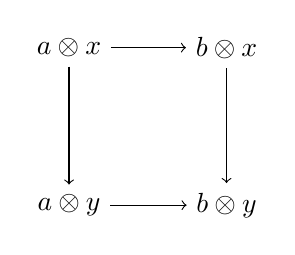
\begin{tikzpicture}
                \node (1) at (0, 0) {$a\otimes x$};
                \node (2) at (2, 0) {$b\otimes x$};
                \node (3) at (0, -2) {$a\otimes y$};
                \node (4) at (2, -2) {$b\otimes y$};
                \draw[->] (1) -- (2);
                \draw[->] (1) -- (3);
                \draw[->] (2) -- (4);
                \draw[->] (3) -- (4);
            \end{tikzpicture}
        \end{gather*}
        The dual concept is sometimes called a \textbf{pullback-hom}, \textbf{pullback-exponential} or \textbf{pullback-power} (depending on which bifunctor is used in the definition). In fact one can drop the requirement that $\mathbf{M}$ carries a monoidal structure and start from any bifunctor $\func{\circledast}{C\times D}{E}$. This more general construction is sometimes called the \textbf{Leibniz construction}.
    }

    \newdef{Monoidal model category}{\index{monoidal!model category}
        A model category $\mathbf{M}$ that carries the structure of closed symmetric monoidal category $(\mathbf{M}, \otimes, \mathbf{1})$ such that the following compatibility conditions are satisfied:
        \begin{enumerate}
            \item \textbf{Pushout-product}: The pushout-product of any two cofibrations is also a cofibration. Furthermore, if any of the two is acyclic, so is the pushout-product.
            \item \textbf{Unit}: For every cofibrant object $x$ and every cofibrant replacement $\widetilde{\mathbf{1}}$ of $\mathbf{1}$, the induced morphism $\widetilde{\mathbf{1}}\otimes x\rightarrow x$ is a weak equivalence.
        \end{enumerate}
    }
    \newdef{Quillen bifunctor}{\index{Quillen!bifunctor}
        Any bifunctor satisfying the pushout-product axiom (where in the definition of the pushout-product we replace the tensor product by the given bifunctor) such that it preserves colimits in both variables is called a \textbf{(left) Quillen bifunctor}. It should be noted that the tensor product automatically satisfies this last property in the case of closed monoidal categories.

        In fact the natural setting for defining Quillen bifunctors is that of two-variable adjunctions \ref{cat:two_variable_adjunction}. Consider such a triple of bifunctors $(\otimes, \text{hom}_L, \text{hom}_R)$.
        \begin{itemize}
            \item The bifunctor $\func{-\otimes-}{C\times D}{E}$ is said to be \textbf{left Quillen} if its pushout-product of cofibrations is again a cofibration, such that acyclicity of one of the domain morphisms leads to acyclicity of the result.
            \item The bifunctors $\text{hom}_L:\mathbf{C}^{op}\times\mathbf{E}\rightarrow\mathbf{D}$ and $\text{hom}_R:\mathbf{D}^{op}\times\mathbf{E}\rightarrow\mathbf{C}$ are said to be \textbf{right Quillen} if its ''Leibniz product'' of a cofibration and a fibration is a fibration, such that acyclicity of one of the domain morphisms leads to acyclicity of the result.
        \end{itemize}
        In fact it can be shown that one of these bifunctors being Quillen implies that the other two are also Quillen.
    }
    \remark{The fact that in the two-variable adjunction approach we do not mention preservation of (co)limits follows from the property that left (resp. right) adjoints preserve colimits (resp. limits).}


\subsection{Enrichment}

    \newdef{Enriched model category}{\index{category!enriched}\index{Joyal-Tierney calculus}
        Let $\mathcal{V}$ be a monoidal model category. A category $\mathbf{M}$ is called a $\mathcal{V}$-enriched model category if is satisfies the following conditions:
        \begin{enumerate}
            \item $\mathbf{M}$ is a $\mathcal{V}$-enriched category that is both powered and copowered over $\mathcal{V}$.
            \item The underlying category $\mathbf{M}_0$ is a model category.
            \item The copower $\cdot:\mathcal{V}\times\mathbf{M}\rightarrow\mathbf{M}$ is a left Quillen bifunctor, or equivalently, the pullback-power (with respect to the $\mathcal{V}$-powering) of any fibration and cofibration (in $\mathbf{M}_0$) is a fibration with respect to the model structure on $\mathcal{V}$ (and it is acyclic if one of the two original morphisms was).\footnote{The fact that the pullback-power axiom is satisfied if and only if the pushout-product axiom is satisfied can be proven by \textit{Joyal-Tierney calculus}.}
        \end{enumerate}
    }

    \newdef{Simplicial model category}{
        A model category enriched over the standard model category of simplicial sets $\mathbf{sSet}_{Quillen}$.
    }

\section{Cofibrant generation}
\subsection{Transfinite constructions}

    We first generalize some notions from ordinary category to the context of regular cardinals $\kappa$:
    \newdef{$\kappa$-filtered category}{\index{category!filtered}
        A  category in which every diagram with less than $\kappa$ arrows admits a cocone.
    }
    \newdef{$\kappa$-directed limit}{\index{limit!directed}
        Consider a poset $I$ such that every subposet of cardinality less than $\kappa$ has a lower bound (upper bound for directed colimits). Such a set is said to be $\kappa$-(co)directed. A limit of a diagram over this poset is called a $\kappa$-(co)directed (co)limit.
    }
    The following definition is a categorification of the previous one:
    \newdef{$\kappa$-filtered limit}{\index{limit!filtered}
        Consider a diagram $\func{D}{I}{C}$. The limit (resp. colimit) of $D$ is said to be $\kappa$-cofiltered (resp. $\kappa$-filtered) if $\mathbf{I}$ is a $\kappa$-cofiltered (resp. $\kappa$-filtered) category.
    }
    It should be noted that an analogue of property \ref{cat:directed_filtered} also holds in the $\kappa$-context, i.e. a category has all $\kappa$-directed colimits if and only if it has all $\kappa$-filtered colimits (and analogously for limits).

    \newdef{Small object}{\index{small}\index{presentable}
        An object for which there exists a regular cardinal $\kappa$ such that its covariant hom-functor preserves all $\kappa$-filtered colimits. These objects are also said to be \textbf{$\kappa$-compact} or \textbf{$\kappa$-presentable}.
    }
    \newdef{Accessible category}{\index{accessible}
        A locally small category $\mathbf{C}$ for which there exists a regular cardinal $\kappa$ such that $\mathbf{C}$ has all $\kappa$-filtered colimits and such that $\mathbf{C}$ contains a set of $\kappa$-small objects that generate all objects by $\kappa$-filtered colimits.
    }
    \newdef{Locally presentable category}{\index{presentable}
        A cocomplete accessible category.
    }

    For ordinary categories the axioms guarantee a (unique) composite of any finite number of (composable) morphisms. However, in some cases it is useful or even necessary to talk about the ''composite'' of an infinite amount of morphisms:
    \newdef{Transfinite composition}{\index{composition}\label{cat:transfinite_composition}
        Consider a category $\mathbf{C}$ with a collection of morphisms $I\subseteq\text{hom}(\mathbf{C})$. Let $\alpha$ be an infinite ordinal\footnote{See definition \ref{set:ordinal} and beyond.}. A ($\alpha$-indexed) \textbf{transfinite sequence} of morphisms in $I$ is a diagram of the form $\func{D}{\alpha}{C}$ such that:
        \begin{enumerate}
            \item Successor morphisms in $\alpha$ are mapped to elements of $I$.
            \item $D$ is \textit{continuous} in the sense that for every limit ordinal $\beta<\alpha$: $D_\beta\cong\underset{\gamma<\beta}{\text{colim}}\ D_{\gamma}$.
        \end{enumerate}
        $D_\lambda$ denotes the restriction of $D$ to the (full) subdiagram $\{\gamma:\gamma<\lambda\}$ of $\alpha$. The transfinite composition of this sequence is the induced morphism $D_0\rightarrow D\alpha\equiv\text{colim}D$.
    }
    \newdef{Cell complex}{\index{cell!complex}
        Consider a cocomplete category $\mathbf{C}$ with a designated set of morphisms $I\subseteq\text{hom}(\mathbf{C})$. A \textbf{relative} $I$-cell complex is a transfinite composition of pushouts of morphisms in $I$. An $I$-cell complex is an object such that the unique morphism from the initial object is a relative $I$-cell complex.
    }
    \newnot{Relative cell complexes}{
        The set of all relative $I$-cell complexes is often denoted by $\text{cell}(I)$.
    }

\subsection{Cofibrant generation}

    We are now ready to state a famous result by \textit{Quillen}:
    \begin{theorem}[Small object argument]\index{small object argument}
        Let $\mathbf{C}$ be a locally presentable category with a designated set of morphisms $I\subseteq\text{hom}(\mathbf{C})$. Every morphism in $\mathbf{C}$ can be factorized as the composition of a morphism in $\text{rlp}(I)$ followed by a morphism in $\text{cell}(I)$.
    \end{theorem}
    \remark{This theorem can be generalized to cocomplete categories where the morphisms in $I$ are small relative\footnote{\textit{Small relative} to a set of morphisms $I$ is defined just as ordinary smallness, but with general $\kappa$-filtered colimits replaced by those that start from morphisms in $I$.} to $\text{cell}(I)$. Sets of morphisms with this property are said to \textbf{admit a small object argument}.}

    \newdef{Cofibrantly generated model category}{\index{model!category}
        Consider a model category $\mathbf{C}$. This category is said to be cofibrantly generated by two sets of morphisms $I,J\subseteq\text{hom}(\mathbf{C})$ if it satisfies the following conditions:
        \begin{enumerate}
            \item $I$ and $J$ both admit the small object argument.
            \item The fibrations are given by $\text{rlp}(J)$.
            \item The acyclic fibrations are given by $\text{rlp}(I)$.
        \end{enumerate}
        It can be shown that the last two conditions are equivalent to the following ones:
        \begin{enumerate}
            \item[$2^*.$] The cofibrations are the retracts (in the arrow category) of $\text{cell}(I)$.
            \item[$3^*.$] The acyclic fibrations are retracts (in the arrow category) of $\text{cell}(J)$.
        \end{enumerate}
        The morphisms in $I$ and $J$ are called the \textbf{generating cofibrations} and \textbf{generating acyclic cofibrations} respectively.
    }

    Sometimes we want our model category $\mathbf{M}$ to have more weak equivalences than it already has. To this end we could try to construct a new model structure $\mathbf{M}_0$. If the cofibrations remain the same then this has some nice properties:
    \begin{itemize}
        \item The fibrations are a subclass of the original ones.
        \item The acyclic fibrations remain the same.
        \item The identity functors $\text{Id}:\mathbf{M}_0\leftrightarrows\mathbf{M}:\text{Id}$ form a Quillen adjunction.
        \item Every object in $\mathbf{M}$ is weakly equivalent (in $\mathbf{M}_0$) to one in $\mathbf{M}_0$.
    \end{itemize}
    We will now make this procedure explicit for a specific class of model categories. Let $\mathbf{M}$ be a left proper, cofibrantly generated simplicial model category and consider a class $S\subset\text{hom}(\mathbf{M})$ of cofibrations with cofibrant domain. First we introduce the notion of ''$S$-local objects'':
    \newdef{Local object}{\index{local!object}
        A fibrant object $x$ is said to be $S$-local if for all morphisms in $S$ their image under its Yoneda embedding is an acyclic Kan fibration. Analogously, a morphism is said to be an $S$-local weak equivalence if for all $S$-local fibrant objects its image under their Yoneda embeddings is an acyclic Kan fibration.
    }
    \begin{property}
        Every weak equivalence is also an $S$-local weak equivalence: $W\subset W_S$.
    \end{property}
    \begin{construct}[Left Bousfield localization]\index{Bousfield localization}
        Given a model category $\mathbf{M}$ with the same assumptions as before, we define the (left) Bousfield localization $L_S\mathbf{M}$ as the same category but with the following model structure:
        \begin{enumerate}
            \item cofibrations: $\text{cof}(L_S\mathbf{M}):=\text{cof}(\mathbf{M})$, and
            \item acyclic cofibrations: cofibrations that are also $S$-local weak equivalences.
        \end{enumerate}
    \end{construct}

    ?? FINISH ??

\section{Homotopy (co)limits}

    Consider a category $\mathbf{C}$ with weak equivalences together with diagrams $\func{F, F'}{I}{C}$. Let us assume that there exists a weak equivalence between $F$ and $F'$, i.e. a natural transformation that consists of componentwise weak equivalences. Clearly this induces a morphism between (co)limits, but it would be nice if the construction of (co)limits would also preserve the homotopy structure, i.e. we want this morphism to be a weak equivalence itself.

    The main purpose of this section is to introduce a correction of the ordinary (co)limit functors to take into account the underlying homotopical structure.

\subsection{Reedy source categories}

    We first consider the general case where we look at diagrams $\func{D}{R}{M}$ where $\mathbf{R}$ is Reedy. We first remark that the constant functor $\func{\Delta}{M}{[R, M]}$ maps weak equivalences to (pointwise) weak equivalences.\footnote{This is clearly also true even when $\mathbf{R}$ is not Reedy.} If the Reedy structure is such that the constant functor preserves cofibrations, then this functor is left Quillen and Ken Brown's lemma \ref{model:ken_brown} implies that its right Quillen adjoint, the limit functor, preserves weak equivalences. In this case we can define the \textbf{homotopy limit} $\text{holim} D$ as the functor $\lim(D\circ Q_f)$ where $Q_f$ is the fibrant replacement-functor (which in this case acts pointwise). A dual construction gives rise to \textbf{homotopy colimits}.

\subsection{Simplicially enriched diagrams}

    In the setting where we consider diagrams in categories enriched over $\mathbf{sSet}$ one can define homotopy (co)limits in a more sophisticated way. References are \cite{hocolim_riehl}. For a refresher on enriched category theory see section \ref{section:enriched_category_theory}.

    \newdef{Homotopy colimit}{
        Consider a diagram $\func{F}{I}{M}$ with $\mathbf{M}$ $\mathbf{sSet}$-enriched. The homotopy colimit of $F$ is defined as the following tensor product:
        \begin{gather}
            \text{hocolim} F := N(-/\mathbf{I})\otimes_{\mathbf{I}}F \overset{\ref{cat:copower_product}}{=} \int^{i\in\mathbf{I}}N(i/\mathbf{I})\cdot Fi.
        \end{gather}
    }
    A similar definition for homotopy limits makes use of a powering:
    \newdef{Homotopy limit}{
        Consider a diagram $\func{F}{I}{M}$ with $\mathbf{M}$ a $\mathbf{sSet}$-enriched model category. The homotopy limit of $F$ is defined as the following hom-like object:
        \begin{gather}
            \text{holim} F := \int_{i\in\mathbf{I}}[N(\mathbf{I}/i), Fi].
        \end{gather}
    }
    \begin{remark}[Bousfield-Kan map]\index{Bousfield-Kan map}
        The expressions from the above formulas are also known as the \textit{Bousfield-Kan formulas}. In fact the above definitions are not quite equivalent to the ones from the previous section. To be precise, the Bousfield-Kan formulas are strictly speaking only weakly equivalent (and hence give satisfying definitions) if we replace the objects in $\mathbf{M}$ by their (co)fibrant replacements, i.e. postcompose $F$ in the above expressions by a (co)fibrant replacement-functor.
    \end{remark}

    ?? COMPLETE ??